%\documentclass[11pt, draft, oneside]{report}
\documentclass[11pt]{report}
\makeindex
\usepackage{ngerman,a4,showidx} %index an seite
%\usepackage{ngerman,a4wide}
%for pdfLaTeX output Bilder als .png speichern:
\usepackage{listings}
\usepackage{nomencl}
\usepackage{framed,color}
\usepackage[pdftex]{graphicx}
% f\"{u}r normales LaTeX->dvi, Bilder als .eps speichern:
\usepackage{graphicx} \DeclareGraphicsExtensions{.eps} %\graphicspath{{bilder/eps/}}

%Definition der Seitengr"osse
\setlength{\textwidth}{15 true cm}
\setlength{\textheight}{22 true cm}
\oddsidemargin  0.5 cm
\evensidemargin 0.5 cm
\topmargin      0 cm

\selectlanguage{german}
%Beispiel fuer ein neues LaTex Kommando
%\newcommand{\QSIM}{{\sc QSim}}


\begin{document}

\begin{titlepage}
\begin{center}
  \vspace*{0.5cm}
  {\LARGE Laborprotokoll Raumakustik LU - Gruppe 4} \\
  \vspace{15mm}
  {\huge \bf Labortag 1 - Messung der Nachhallzeit \\}

  \vspace{15mm}
  {\LARGE Andreas Johann H\"ormer\\
Name 2} \\

  \vspace{10mm}%15
  -------------------------------------- \\
  \vspace{10mm}%15
  \large
  Institute for signal processing and speech communication \\
  Graz University of Technology \\


  %Vorstand: O.\,Univ.-Prof.\,Dipl.-Ing.\,Dr.\,techn.\,Reinhold Wei{\ss} \\
  \vspace{15mm}%1
  \begin{figure}[!ht]
  \begin{center}
  \centerline{
\includegraphics[width=4cm,keepaspectratio=true]{TULogoneu}}
  \end{center}
  \end{figure}
  \vspace{10mm}
Laborbetreuung: DI\,Dr.\,techn. Franz Graf \\
  %Begutachter: O.\,A.o.Univ.-Prof.\,Dipl.-Ing.\,Dr.\,techn.\,Eugen Brenner \\
  %\vspace{5mm}
  %Betreuer: Univ.-Ass. Dipl.-Ing.\,Dr.\,techn.\,N. N.\\
  \vfill
  %\newline
  %\normalsize
  Tonstudio TU Graz, 27.04.2015
  \vspace{0.5cm}
\end{center}
\end{titlepage}

% Die Titelseite ist immer in Deutsch (austrian), danach h\"{a}ngt es von der
% Sprache der Diplomarbeit ab. Jedenfalls muss eine Kurzfassung und
% ein Abstract existieren

%\thispagestyle{empty} 
%\selectlanguage{english}


\newpage
\selectlanguage{german}
%\vspace*{2.2 cm}
%{\Large
%\noindent
%{\bf Abstract}} \\
%\vspace*{0.3 cm}

%\noindent
%Main target of this laboratory was the measurement of different DACs and ADCs of the fully digital mixing panel LAWO $mc^2 66$. Additionally preamplifiers of a %high quality input compared to standard inputs were measured. Measurements were done qualitatively in terms of dynamic ranges and frequency characteristics.%\\
%This report consists of 28 pages. 


%\newpage


%\selectlanguage{english}
%\vspace*{2.2 cm}
%{\Large
%\noindent
%{\bf STATUTORY DECLARATION}} \\
%\vspace*{0.3 cm}

%\noindent
%I declare that I have authored this thesis independently, that I have not used other than the declared sources / %resources, and that I have explicitly marked all material which has been quoted either literally or by content from %the used sources.
%\vspace*{0.3 cm}

%\vspace{2 cm}

%\noindent ..............................\hfill ...........................................


%\noindent date  \hfill (signature)
\renewcommand{\nomname}{List of abbreviations}
\setlength{\nomlabelwidth}{.50\hsize}
\renewcommand{\nomlabel}[1]{#1 \dotfill}
\setlength{\nomitemsep}{-\parsep}
\makenomenclature

\newpage
\selectlanguage{german}
%\newpage
%\vspace*{2.2 cm}
%{\Large
%\noindent
%{\bf Danksagung}} \\
%\vspace*{0.3 cm}
% OPTIONAL

%\noindent
%Diese Diplomarbeit wurde im (Studien)Jahr am Institut f\"{u}r
%Technische Informatik an der Technischen Universit\"{a}t Graz
%durchgef\"{u}hrt.

%\smallskip
%Danksagung an alle am Institut bzw. bei Firmen, die geholfen
%haben....

%\medskip
%Danksagung an Freunde und Freundinnen f\"{u}r das Verst\"{a}ndnis, ebenso
%den Eltern und allen sonstigen Sponsoren....

%\vspace{2 cm}

%
%\noindent Graz, im Monat Jahr \hfill Name des Diplomanden

\newpage
% Inhaltsverzeichnis
\tableofcontents  

% Tabellenverzeichnis
% OPTIONAL
%




\listoffigures 

% Abbildungsverzeichnis
% OPTIONAL
%\listoftables

%Seitennummerierung am Kopf inkl. Kapitel"uberschrift
\pagestyle{headings}

%---------------------------------------------------------------------------------------------------------
%---------------------------------------------------------------------------------------------------------

\chapter{Messung der Nachhallzeit}
\section{Messung im Aufnahmeraum AR}
\subsection{Messung mittels Methode des abgeschalteten Rauschens}
\subsection{Impulsmessung}
\section{Messung im Hörsaal i2}
\subsection{Impulsmessung}


%\begin{figure}[htbp]
%\begin{center}
%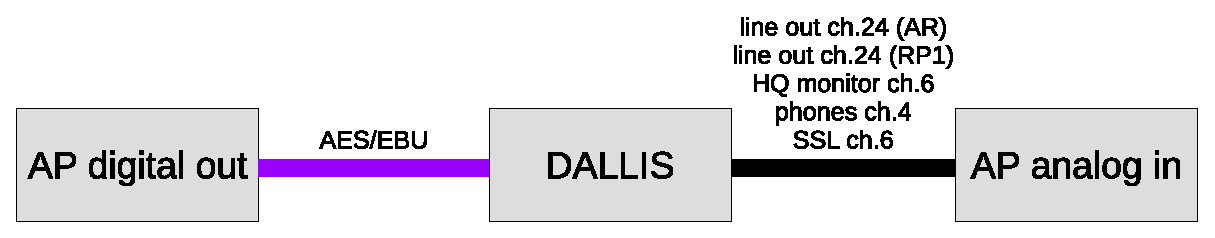
\includegraphics[width=14cm,keepaspectratio=true]{DACstructure}
%\caption{experimental setup for DAC measurement}
%\label{fig:dacstructure}
%\end{center}
%\end{figure}

%\begin{table}
%\begin{center}
%\begin{tabular}{|c||c|c|}
%\hline 
%output channel  & 	output level [$dB_{FS}$]&		input level [$dB_u$]\\ \hline
%line out ch.24 (AR) &	-18 &	+6\\
%line out ch.24 (RP1) &	-18 &		+6\\
%HQ monitor ch.6 &	-9 		& +6\\
%phones ch.4 &	-15 &	+6\\
%\hline
%\end{tabular}
%\caption{values for output and input levels for DAC measurements}
%\label{tab:dacvalues}
%\end{center}
%\end{table}
%\begin{leftbar}
%\textit{ Note:\\
%A measurement of phase shifts is not possible when driving the system with a digital output signal.}
%\end{leftbar}

\end{document}
